% !TeX spellcheck = en_US
\section{Characterization of Video Content}
 \label{sec:724_videoClassification}
\subsection{Idea of the Categorization}
The main contribution proposed in this section is the reuse of existing quality models generated for a specific video for other videos. 
To understand which existing quality model should be used for an unknown video, \ac{VAS} classifies videos.
It is assumed that videos in the same class have similar quality models, and thus require similar quality adaptations.
A classification of the video characteristics simplifies quality estimation.

The classes are characterized by visual features that represent the video content.
To reduce \ac{VAS}'s operational costs, these features should be much easier and faster to produce in comparison to the execution of \ac{VQM}. % on \ac{CPU}s.
To support live video streaming scenarios, a real-time calculation of the features is necessary.
\subsection{Features for Classification}
 \label{sec:724_calculationSITI_Structures}
We select features which are inspired by existing knowledge of the human visual system.
As mentioned above, the features that are selected represent the structures in a video frame (\ac{SI}), the motion between video frames (\ac{TI}) and the colorfulness (\ac{Co}) of a video~\cite{ITU-J2008,Winkler2012}. 
These characteristics, which are calculated for each video chunk, are analyzed as they indicate how the human vision system perceives video quality~\cite{Winkler2012}. 
 %\subsubsection{Structural Intensity}}.
The \ac{ITU} recommendation has shown that specific metrics are reliable for classifying short video sequences in the context of subjective video estimations.
\ac{VAS} leverages the recommendations of the \ac{ITU}, which are introduced for the video composition application in Section~\ref{sec:630_autocompose} for \ac{SI}, \ac{TI}, and \ac{Co}~\cite{ITU-J2008}.
These metrics are calculated for individual video shots. %  -  the video shot or the \ac{DASH} segment.
\ac{VAS} leverages the metrics to select appropriate quality models from the \ac{VAS} database.
It stores for each video shot the content characteristics along with the generated quality models.
An advantage of \ac{SI}, \ac{TI}, and the quality estimator \ac{VQM} is that they share a Sobel filter calculation to detect edges.
Thus, a Sobel-filtered video frame can be reused in multiple processing steps.
\subsection{Selection of Characteristics}
\label{sec:724_selection}
Based on this classification, suitable adaptation plans are generated as \ac{VAS} assumes that perceived quality differences of video representations encoded with the same resolution, frame rate, and bit rate are similar if the \ac{SI}, \ac{TI}, and \ac{Co} values of the video shots are similar.
The calculated adaptation plans, available video representations, and \ac{SI}, \ac{TI}, and \ac{Co} profiles of a video are stored in a database of \ac{VAS} (see Figure~\ref{fig:720_architecture}). 
The stored combinations are used to ensure the timely calculation of adaptation plans. 
 As it cannot be guaranteed that video quality estimation of different representations can be achieved in time in any situation, previous quality estimations and their \ac{SI}, \ac{TI}, and \ac{Co} values are stored in the database. 
 
 Unknown video sequences can be classified solely based on retrieving the \ac{SI}, \ac{TI}, and \ac{Co} profiles. 
 The profiles are then compared via nearest-neighbor matching (i.e., Euclidian distance of SI, TI and Co values) with existing profiles from the \ac{VAS} database. 
 To select an appropriate video shot from the database, the closest match is determined by the Euclidian distance:
 \begin{equation}
 ED_{SI,TI,Co}=\sqrt{(SI_{\text{DB}} - SI_{\text{Video}})^2 + (TI_{\text{DB}} - TI_{\text{Video}})^2 + (Co_{\text{DB}} - Co_{\text{Video}})^2}
 \end{equation}
 In this equation, $SI_{\text{DB}}$ represents the SI value for a video shot stored in the \ac{VAS} database, whereas $SI_{\text{Video}}$ represents the respective value of the currently played-back video stream.
 The aim is to minimize $ED_{SI,TI, Co}$ and to choose the reference with the smallest difference to predict the adaptation behavior.
 The adaptation plans of the match in the database are applied to the new video sequence. 
 
The Euclidian distance weighs all features (SI, TI and Co) equally and does not prioritize any feature.
Winkler et al. report that no clear preference to a feature can be given when classifying video content~\cite{Winkler2012}.
 
This is the basis for selecting an appropriate adaptation plan based on the perceived quality, as shown in Subsection~\ref{sec:726_adaptationstrategy}.
In the preprocessing stage, the \ac{SI}, \ac{TI}, and \ac{Co} calculations can be massively parallelized across different video shots and different representation combinations. 
\subsection{Video Characteristics and Quality Models}
The assumption is that \ac{MPEG} \ac{DASH} videos showing similar content have alike quality models, and thus benefit from the same adaptation plans.
\subsubsection{Quality Model Prediction Error}
\label{sec:724_quality_model_prediction_error}
The assumption that \ac{VAS} can use existing quality models from videos with similar content characteristics is validated by investigating the average error when conducting such a mapping.
For a video shot, the average error regarding the \ac{DMOS} shows the average, absolute distance between another shot's quality model with a similar \ac{SI}, \ac{TI}, and \ac{Co} profile and the \ac{MOS} predicted by \ac{VQM}.
The similarity between the video shots is measured using the Euclidian distance, as described for \ac{VAS} in Section~\ref{sec:724_selection}. 
The videos from the \ac{MPEG} \ac{DASH} dataset - provided by University of Klagenfurt, Austria - are used for validating the assumption~\cite{Lederer2012a,Lederer2013}.
The dataset contains seven long-running videos encoded in 17 to 19 representations from \ac{240p} to \ac{1080p} resolution.
All \ac{MPEG} \ac{DASH} representations of a video have the same frame rate.
The characteristics of this \ac{MPEG} \ac{DASH} dataset are extensively discussed in Section~\ref{sec:730_video_dataset}.

The complete preprocessing stage is applied to all representations of all videos in the dataset to retrieve the \ac{SI}, \ac{TI}, and \ac{Co} profiles and quality models for all video shots.
Figure~\ref{fig:plotvalidationoferroreucliddmos2all} depicts the average error when predicting a quality model for a video shot in relation to the Euclidian distance of both the predicted and the real quality model.
\begin{figure}[tbh]
\centering
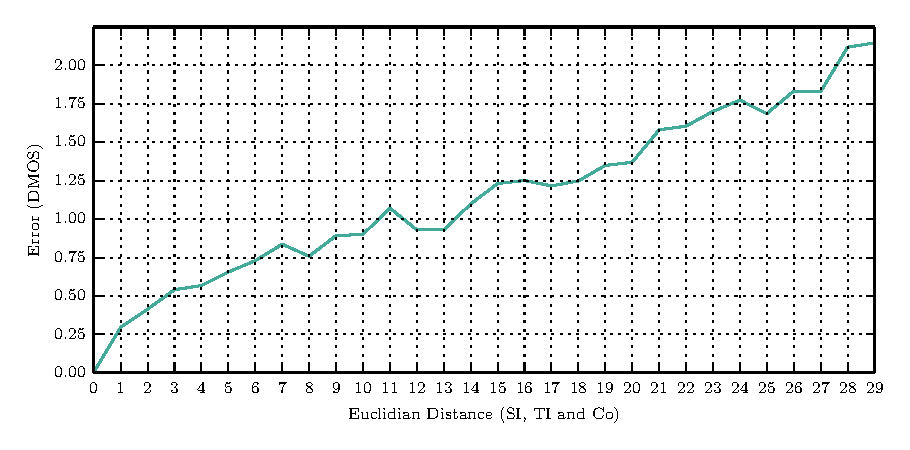
\includegraphics{gfx/700_VAS/plotValidationOfErrorEUCLID_DMOS2_ALL}
\caption[Average errors in the prediction of quality models]{Average error for the prediction of a quality model with similar content characteristics.}
\label{fig:plotvalidationoferroreucliddmos2all}
\end{figure}

If a shot can be found with exactly the same content characteristics, the quality model fits best. 
In this case, the average error is close to zero and below any noticeable difference for a human observer.
With increasing distance, the error also increases. 
This shows that a single quality model is not suitable for all video shots. 
Up to an Euclidian distance of approximately 10.5, the average error stays below a \ac{DMOS} of 1. 
Still, \ac{VAS} needs to find similarly encoded video shots, where the average distance of content characteristics is as small as possible.
Euclidian distances below 3 lead to only negligible deviations from the correct quality model.
\subsubsection{Influence of Video Dimensions on Reliability}
Content characterization is further beneficial if the necessary calculations are made as quickly as possible.
One possibility to reduce processing time is to limit the maximum resolution, bit rate and frame rate of the video. 
\begin{figure}[!tbh]
\centering
\subfloat[]{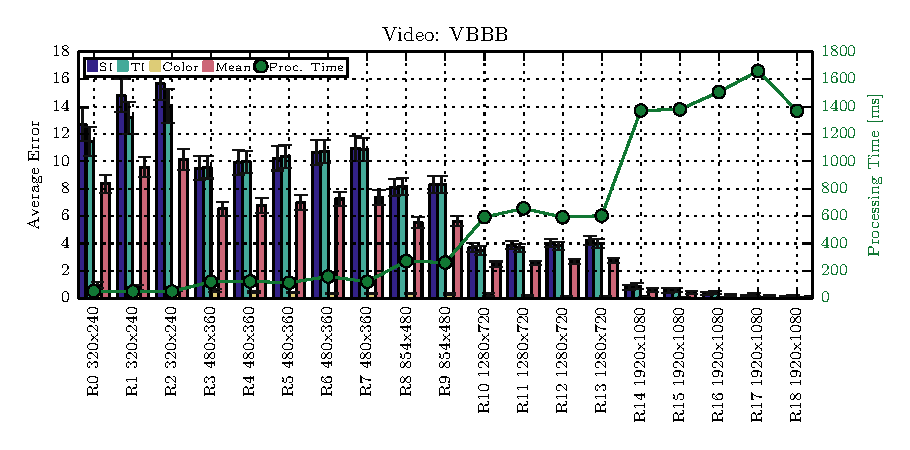
\includegraphics{gfx/700_VAS/siti_error_VBBB}}\\
\subfloat[]{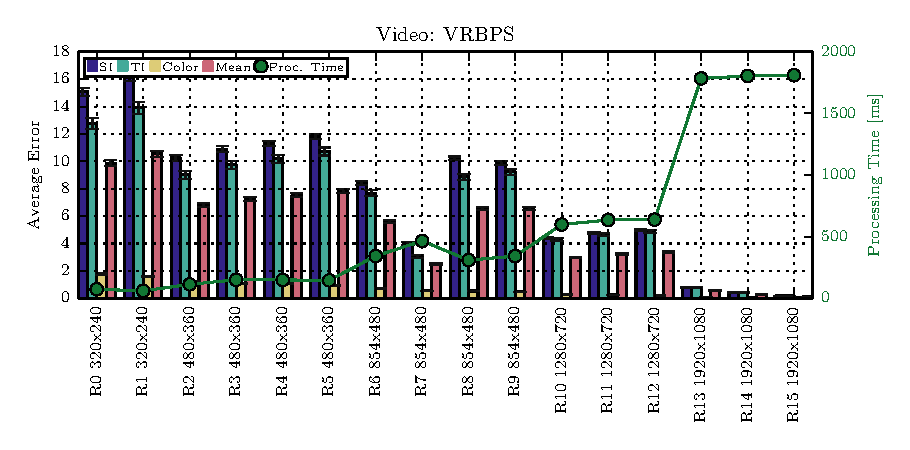
\includegraphics{gfx/700_VAS/siti_error_VRBPS}}
\caption[Average error for calculating the \ac{SI}, \ac{TI} and \ac{Co} characteristics]{Average error for predicting the \ac{SI}, \ac{TI} and \ac{Co} characteristics at low bit rate \ac{MPEG} \ac{DASH} representations for the (a) VBBB and (b) VRBPS videos.}
\label{fig:sitierrorvbbb}
\end{figure}

The \ac{SI}, \ac{TI}, and \ac{Co} profiles can be calculated not only from the highest representation but also from any other.
The question arises: how inaccurate are calculations when a lower representation is chosen? 
Using the ITEC \ac{MPEG} \ac{DASH} dataset from Klagenfurt, the error in predicting the \ac{SI}, \ac{TI}, and \ac{Co} values is calculated.
The reference is the highest available representation, which is not depicted in the graphs.
The representations are sorted by an increasing resolution and bit rate, meaning, that two representations with similar resolutions differ regarding the quantization used for encoding. 
The frame rate is held stable as a decrease in frame rate results in a high average error for predicting the video's \ac{TI} characteristics.
Results are depicted in Figure~\ref{fig:sitierrorvbbb} for the videos VBBB and VRBPS, which can be mapped to all other videos in the dataset.
The processing time is calculated based on the sequential processing of the \ac{SI}, \ac{TI}, and \ac{Co} on a single dedicated \ac{CPU} core of an Intel Xeon CPU E5-1650 v2 @ 3.50GHz for one second of video.

The results illustrate that an increase in the resolution significantly reduces the prediction error but a linear relation between the resolution and the processing time exists.
The quantization or bit rate has no significant (95\% confidence intervals) impact on the processing time, but it slightly reduces the average error (red bar) as more details can be encoded. 
The increased processing time is a result of the data increase that needs to be loaded from the hard disk to the memory.
A resolution of \ac{720p} for a \ac{1080p} reference video, or \ac{360p} for a \ac{576p} reference video, sufficiently shows both low prediction errors and more than half on the required processing time.
These findings coincide with the results on the reliability of extracting other visual features from lower resolution videos as described by Manweiler et al.~\cite{Manweiler2012}.

It can be concluded that a classification of \ac{MPEG} \ac{DASH} videos can be quickly and reliably done for low resolutions, and a complete quality model can be mapped by only inspecting a single \ac{MPEG} \ac{DASH} representation.